\scanpage{56}
\mspage{2}
% archive foliation: 58
ment en série qui commence par
\[
a_nz^n\qquad n>0,\ a_n\ne0\qquad(\text{OPS }x=0)
\]
on voit tout de suite que l'on doit avoir
$n=1$ ---

\margin{Notes : \uline{indétermination} \uline{\unsure{finie}} d'une carte loc.
au bord : modulo chgt. de coordonnées par un \unsure{germe}
de fct. analytique \uuline{\unsure{réelle|nulle}}.}

\noindent$\bigl[$\uline{Thm 2} Équiv. de la cat. des surfaces conformes
à bord \inserted{compactes}, avec celle des courbes alg. propres
lisses sur $\mathbb R$. $\bigr]$

\margin{\uline{NB} À partir d'ici $H$ désigne le demi-plan \uline{fermé}
$\{\deleted{\unsure{\mathbb R}}z\in\mathbb C\mid\Im z\geq0\}$.}

\textcircled{2)} Découpe d'une surface conforme à bord,
suivant un 1-complexe top. $K\subset X$,
satisfaisant des hypothèses de régularité
convenables (rectifiabilité suffit ?).

\uline{Théorème 3} La découpe $\widetilde X$, muni de \deleted{la}
\deleted{structure}\inserted{faisceau} des fonctions \inserted{complexes} continues conformes
dans $\operatorname{Int}(\widetilde X)$ $(\simeq X\setminus K)$, ``est'' une surface
conforme à bord.

\margin{C'est un th. du type ``uniformisation \uline{à bord}''.}

Cela revient à vérifier \deleted{donc} que \inserted{pour} tout
point $\unsure{\widetilde x|\overline x}$ de $\delta\widetilde X$, il existe un voisinage \inserted{ouvert} $U$ de $x$,
et un \deleted{\unsure{isom}}\inserted{homéo} de $U$ avec $H\cap\mathbb D^\circ$ (où
$\mathbb D=\{z\in\mathbb C\mid |z|\leq1\}$ est le disque
unité de $\mathbb C$). Cela revient

\margin{\unsure{renv. mt}\ \unsure{dans a)} Cor. au théor.}

\figure{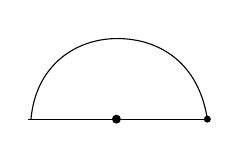
\begin{tikzpicture}[scale=.7]
\draw (-1.7,0) .. controls (-1.6,1.15) and (-.6,1.65) .. (.35,1.4)
.. controls (1.05,1.2) and (1.4,.65) .. (1.5,0);
\draw (-1.75,0)--(1.5,0);
\fill (-.15,0) circle (2.3pt);
\fill (1.5,0) circle (1.8pt);
\end{tikzpicture}}

à deux choses, suivant que $x$ correspond :
